\testsection{Bar diagrams}
{
\pgfkeys{/pgfplots/bar style/.style={%
		/pgfplots,
		%legend style={cells={anchor=base}},
		legend image code/.code={\draw[##1,yshift=-0.2em] plot coordinates {(0cm,0.8em)};},
	}
}%
\begin{tikzpicture}
	\begin{axis}[
		%xmin=1925,xmax=1975,disabledatascaling=false,
		%xtick={1930,1940,1950,1960,1970},
		x tick label style={/pgf/number format/set thousands separator=},
		ylabel=Population,
		legend style={at={(0.5,-0.1)},anchor=north,legend columns=-1},
	]
	\addplot[ybar,draw=blue,mark=none,fill=blue!80!black] 
		plot coordinates {(1930,50e6) (1940,33e6) (1950,40e6) (1960,50e6) (1970,70e6)};
		%plot coordinates {(1933,5) (1945,3) (1950,4) (1965,5) (1980,7)};
	\addlegendentry[bar style]{FarFarAway}

	\addplot[ybar,xshift=6pt,mark=none,red,fill=red!80!black] 
		plot coordinates {(1930,38e6) (1940,42e6) (1950,43e6) (1960,45e6) (1970,65e6)};
	\addlegendentry[bar style]{NotSoFar}

	\addplot[ybar,xshift=12pt,mark=none,brown,fill=brown!80!black] 
		plot coordinates {(1930,15e6) (1940,12e6) (1950,13e6) (1960,25e6) (1970,35e6)};
	\addlegendentry[bar style]{Near}
	\end{axis}
\end{tikzpicture}
}

\testsubsection{const plot}
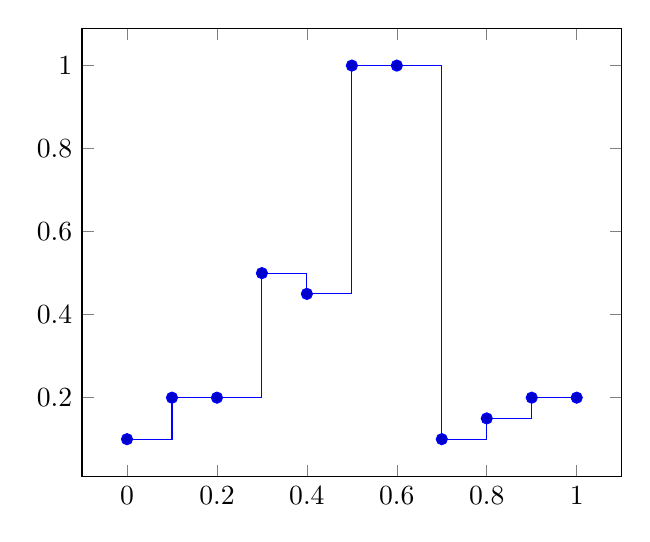
\begin{tikzpicture}
	\begin{axis}
	\addplot+[const plot]
		coordinates {(0,0.1) (0.1,0.2) (0.2,0.2) (0.3,0.5) (0.4,0.45) (0.5,1) (0.6,1) (0.7,0.1) (0.8,0.15) (0.9,0.2) (1,0.2)};
	\end{axis}
\end{tikzpicture}

\testsubsection{jump mark right}
\begin{tikzpicture}
	\begin{axis}
	\addplot+[jump mark right]
		coordinates {(0,0.1) (0.1,0.2) (0.2,0.2) (0.3,0.5) (0.4,0.45) (0.5,1) (0.6,1) (0.7,0.1) (0.8,0.15) (0.9,0.2) (1,0.2)};
	\end{axis}
\end{tikzpicture}

\testsubsection{jump mark left}
\begin{tikzpicture}
	\begin{axis}
	\addplot+[jump mark left]
		coordinates {(0,0.1) (0.1,0.2) (0.2,0.2) (0.3,0.5) (0.4,0.45) (0.5,1) (0.6,1) (0.7,0.1) (0.8,0.15) (0.9,0.2) (1,0.2)};
	\end{axis}
\end{tikzpicture}
